\documentclass[a4paper]{report}

\usepackage{generalsnips}
\usepackage{calculussnips}
\usepackage[margin = 0.80in]{geometry}
\usepackage{pdfpages}
\usepackage[spanish]{babel}
\usepackage{amsmath}
\usepackage{amsthm}
\usepackage[utf8]{inputenc}
\usepackage{titlesec}
\usepackage{xpatch}
\usepackage{fancyhdr}
\usepackage{tikz}
\usepackage{float}
\usepackage{multicol}
\usepackage{wrapfig}
\usepackage{blindtext}
\usepackage{array}
\usepackage{enumitem}
\usepackage{url}
\usepackage{breakurl}
\usepackage{hyperref}

\decimalpoint
\begin{document}
\sloppy
\begin{titlepage}
    \begin{center}
        \thispagestyle{empty}
        \renewcommand{\headrulewidth}{0pt}
        \renewcommand{\footrulewidth}{0pt}
        
        \begin{tabular}{ p{0.5\textwidth}p{0.5\textwidth} }
            \begin{flushleft}
                Facultad de Ciencias Económicas \\
                Universidad Francisco Marroquín \\
                Statistical Thinking II \\ 
                Catedrático: Eugenio Aristondo \\ 
                Auxiliar: Paulo Mejía \\
                Guatemala \\
                15 de noviembre de 2020 \\ 
            \end{flushleft}
            &
            \begin{flushright}
                
\includegraphics[width=0.5\textwidth]{./appendages/ufmlogo.png} \\ 
            \end{flushright} \\ 
        \end{tabular}
        
            
        \cfoot{} % this is to remove the page number
        \vspace*{7cm}
        {
            \Huge Diferencia de poblaciones: aumentos de Dopamina de acuerdo al instrumento musical tocado
        }
 
        \vspace{1.5cm}

 
        \vfill
             
        \vspace{0.8cm}
        
        
        \begin{flushleft}
            \begin{tabular}{ ll }
                Anesveth Maatens & 20190339 \\
                Andrea Reyes     & 20190265 \\
                David Corzo      & 20190432 \\
                Daniel Cabrera   & 20190069 \\
                Fabricio Juárez  & 20190361 \\ 
            \end{tabular}
        \end{flushleft}     
    \end{center}
\end{titlepage}

%%%%%%%%%%%%%%%%%%%%%%%%%%%%%%%%%%%%%%%%%%%%%%%%%%%%%%%%%%%%%%%%%%%%%%%%%%%


\section{Introducción}
% \subsection{Marco teórico}
Tocar un instrumento tiene muchos beneficios, entre ellos, el empezar a hacerlo a una corta edad puede ayudar en la memoria, cognición y otros beneficios en un futuro [1]. La dopamina, es uno de varios neurotransmisores que utilizan las neuronas para comunicarse entre ellas. La dopamina es considerada como la causante de sensaciones placenteras y de relajación. El cerebro libera dopamina cuando una persona escucha música que le parece agradable e incluso, cuando sabe que la escuchará en el futuro cercano [2]. La música contribuye a disminuir la ansiedad, mejorar la frecuencia cardiaca y el humor, por estas y más ventajas, la música se usa cada vez más como herramienta terapéutica [2]. 
Como hemos mencionado antes, si al escuchar música se producen efectos positivos en nuestro cuerpo, el interpretar música o tocar un instrumento producen aún más, ya que al tocar, no solo se está escuchando música sino que también se pone en acción la coordinación de la mente y el cuerpo.

La música es considerada uno de los elementos que causan más placer en la vida ya que, como hemos mencionado anteriormente, ayuda a estabilizar las emociones debido a la liberación de dopamina y otros neurotransmisores. Otra función a cargo de la dopamina es regular la captación de la información, en otras palabras, los recuerdos y la memoria [3]. Si la información que entra a nuestro cerebro no nos gusta, el hipocampo no se activa y el recuerdo no se almacena en la memoria, es por eso que los músicos tienden a tener una mejor memoria [3]. El hipocampo es una de las partes del cerebro que está situado en el sistema límbico. Está relacionado tanto con los procesos mentales relacionados con la memoria como con los procesos de producción y regulación de estados emocionales. El hipocampo permite que la información pase a la memoria a largo plazo conectando la información recibida con valores positivos o negativos dependiendo de si los recuerdos son placenteros o dolorosos [3].

La música es procesada por ambos hemisferios. El hemisferio derecho recibe el estímulo musical y el hemisferio izquierdo interpreta y controla la información. En conclusión, tocar un instrumento estimula el cerebro de tal manera que es capaz de poner a trabajar ambos lados o hemisferios del cerebro y liberar sustancias que ayudan a liberar sensaciones negativas y reemplazar esas sensaciones por placer y felicidad [3].


\vspace{0.5cm}
%----------------------------------------------------------------------------------------
% \subsection{Relevancia del estudio}
Este estudio es de gran relevancia ya que al obtener resultados e información sobre el efecto causado en el aumento o disminución de la dopamina al tocar un instrumento, se pueden hacer recomendaciones a instituciones dedicadas a la salud emocional y a personas con necesidad de mejorar su estado de ánimo, estrés y humor. Incluso, con los resultados posibles de este estudio, se pueden recomendar instrumentos en específico, con indicaciones sobre qué instrumento aumenta más la secreción de dopamina al tocarlo.



\vspace{0.5cm}
%----------------------------------------------------------------------------------------
% \subsection{Objetivos}
El objetivo principal de la investigación fue tomar muestras de dopamina entre personas seleccionadas aleatoriamente antes y después de tocar tres tipos de instrumentos, esto para demostrar si existe o no una diferencia estadísticamente significativa en el aumento de dopamina  al  tocar piano, cello o flauta.


\vspace{0.5cm}
%----------------------------------------------------------------------------------------
% \subsection{Hipótesis de investigación}
Se analizó tres diferentes instrumentos para comprobar si existe diferencia estadísticamente significativa entre el nivel de dopamina que segrega cada una de ellos, y determinamos como hipótesis nula la proposición: ``No existe diferencia estadísticamente significativa  en el aumento de dopamina entre tocar piano, cello o flauta''; y como hipótesis alternativa la proposición que ``Sí existe diferencia estadísticamente significativa  en el aumento de dopamina entre tocar el piano, cello o flauta''. 

\vspace{0.5cm}
%----------------------------------------------------------------------------------------
% \subsection{Justificación del proyecto}
Con el marco teórico previo, se puede afirmar que tocar música tiende a aumentar el nivel de dopamina en el cerebro de un individuo. De aquí, nace la interrogante de si el instrumento que se toca afecta en alguna manera la cantidad producida. Por esto, se pretende con esta investigación evaluar si existe una diferencia estadísticamente significativa entre los niveles de dopamina que generan los tres instrumentos analizados.


%----------------------------------------------------------------------------------------


\section{Descripción del experimento}
El experimento consta de una serie de pruebas estadísticas hechas a tres poblaciones distintas: una población de personas que tocan el cello, otra que toca la flauta y otra que toca el piano. Las muestras provienen de tomar la medición de dopamina antes y después de tocar el instrumento asignado, puesto a que lo que nos interesa es el aumento o disminución que cause tocar el instrumento se determinó pertinente tomar las diferencias entre la medición posterior a tocar el instrumento y la medición previa a tocarlo.


Pruebas a realizar: 
\begin{itemize}
    \item La primera prueba fue utilizada para comparar los aumentos o disminuciones de las tres poblaciones (Piano, Flauta, Cello) para esto utilizamos la prueba de hipótesis no paramétrica Kruskal-Wallis. (Además condujimos dos pruebas más para dar refuerzo estadístico a esta prueba.)
    \item La segunda prueba fue utilizada para analizar si existe una diferencia estadística entre los niveles de dopamina entre las poblaciones que tocan el piano y los que tocan el cello. Mann-Whitney-Wilcoxon y comparar si estos resultados son congruentes a la prueba anterior (Kruskal-Wallis).
    \item La tercera prueba fue realizada para analizar si existe diferencia estadísticamente significativa entre las diferencias de los niveles de dopamina antes y después de tocar el instrumento respectivo. Para esta prueba se utilizaron las poblaciones que tocan Cello y Piano y se determinó pertinente usar la prueba Mann-Whitney-Wilcoxon, además comparar si los resultados provenientes de esta prueba apoyaban o no a los resultados concluidos en la primera prueba (Kruskal-Wallis).
\end{itemize}


\section{Procedimientos o métodos}
\subsection{Ejecución de prueba Kruskal-Wallis para comparar las diferencias entre la dopamina segregada antes y después de tocar Piano, Cello y Flauta}
A continuación se encuentran las diferencias entre la medición de dopamina de personas seleccionadas aleatoriamente antes de tocar un instrumento y después de tocar un instrumento, la resta de las mediciones antes de tocar instrumentos y después produjeron la siguiente tabla.

Es importante considerar lo siguiente: 
\begin{itemize}
    \item Cuando los datos son negativos significa que el nivel de dopamina después de tocar un instrumento disminuyó en comparación al nivel de dopamina antes de tocar un instrumento.
    \item Cuando los datos son 0 significa que el nivel de dopamina se mantuvo constante durante el experimento. 
    \item Cuando los datos son positivos significa que al tocar dicho instrumento la dopamina aumentó en comparación al nivel de dopamina segregada antes de tocar el instrumento.
\end{itemize}

Queremos investigar si el nivel de dopamina segregado después de tocar alguno de los instrumentos en cuestión (piano, cello o flauta) es diferente según cuál instrumento se esté tocando.

\begin{center}
    \begin{tabular}{ |ccc| }
        \hline  
            PIANO & CELLO & FLAUTA \\ 
        \hline
            0.5 & 0.3 & 0.6  \\
            0.1 & 0.4 & 0.1   \\
            -0.1 & 0.5 & 0.1   \\
            -0.3 & 0.3 & 0   \\
            -0.4 & 0.3 & -0.9   \\
            1.2 & -0.1 & -0.5   \\
            -0.4 & 0.2 & 0.3   \\
            -0.2 & 0.4 & 0.7   \\
            -0.7 & 0.2 & 0.6   \\
            0 & 0.4 & 0  \\
            -0.6 & 0.9 & 0.3   \\
            -0.5 & 0 & -0.1  \\ 
        \hline
    \end{tabular}
\end{center}

Por la naturaleza del experimento procederemos a aplicar la prueba Kruskal-Wallis para comparar las tres poblaciones.

\begin{enumerate}
    \item Justificación de la prueba: 
        \begin{itemize}
            \item $n_{1,2,3} \geq 5$
            \item Puesto al hecho que tenemos que comparar varias poblaciones procedemos a usar esta prueba. 
        \end{itemize}
    \item Estadístico de prueba: poblaciones.
    \item Hipótesis: 
        \begin{enumerate}
            \item $H_0$: todas las poblaciones son iguales. %$\text{población}_1 = \text{población}_2 = \text{población}_3$.
            \item $H_a$: no todas las poblaciones son iguales. %$\text{población}_1 \neq \text{población}_2 \neq \text{población}_3$.
        \end{enumerate}
    
    \item Significancia: $\alpha = 0.05$
    \item Estadístico de prueba: 
        \begin{itemize}
            \item Establecemos las variables preliminares:  
                \begin{itemize}
                    \item $k=3$ (3 muestras).
                    \item $n_P = 12, \qq n_C = 12, \qq n_F = 12$ ($n_P$ númbero de observaciones de piano, $n_C$ número de observaciones de cello, $n_F$ número de observaciones de flauta).
                    \item $n_T = 36$ (número total de observaciones).
                    \item $R_P = 149.5, \qq R_C = 288, \qq R_F = 288.5 $ ($R_P$ suma de rangos de piano, $R_C$ suma de rangos de cello, $R_F$ suma de rangos de flauta).
                        \begin{center}
                            \begin{tabular}{|lll|}
                                \hline
                                PIANO & CELLO & FLAUTA \\
                                \hline
                                30.5 & 24 & 32.5 \\
                                18 & 28 & 18 \\
                                11 & 30.5 & 18 \\
                                8 & 24 & 14.5 \\
                                6.5 & 24 & 1 \\
                                36 & 11 & 4.5 \\
                                6.5 & 20.5 & 24 \\
                                9 & 28 & 34 \\
                                2 & 20.5 & 32.5 \\
                                14.5 & 28 & 14.5 \\
                                3 & 35 & 24 \\
                                4.5 & 14.5 & 11 \\
                                \textbf{149.5} & \textbf{288} & \textbf{228.5} \\
                                \hline
                            \end{tabular}
                        \end{center}
                    
                    \item $gl=2$ (grados de libertad para $\chi^2$). 
                    \item $\displaystyle \sum_{i=1}^{k}\frac{R^2_i}{n_i} = 13125.54167$
                        \[
                            \sum_{i=1}^{3} \frac{R^2_i}{n_i} = \p{\frac{149.5^2}{12}}  + \p{\frac{288^2}{12}}  + \p{\frac{288.5^2}{12}}  =  13125.54167 \\ 
                        \]
                \end{itemize}
            
            \item Procedemos a calcular el estadístico $H = 7.248123123$. 
                \begin{center}
                   \begin{align*}
                       H &= \sqb{\frac{12}{n_T(n_T+1)}\sum_{i=1}^{k}\frac{R^2_i}{n_i}} -3(n_T+1) \\ 
                       &= \sqb{\frac{12}{36 \times (36 + 1)}\times 13125.54167} -3\times(36 + 1) \\ 
                       &= \sqb{0.009009009 \times 13125.54167} -111 \\ 
                       &= 7.248123123 \\ 
                   \end{align*}
                \end{center}
            
            \item Procedemos a sacar el $valor-p = 0.026674118$:
                \begin{figure}[H]
                    \centering
                    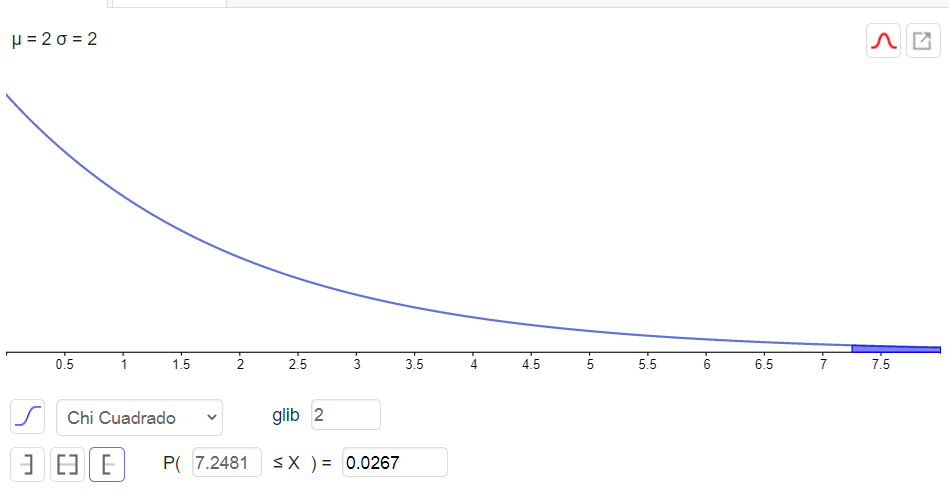
\includegraphics[width=0.8\textwidth]{./appendages/valor-pKW.png}
                    \caption{Geogebra: sacado de la calculadora de probabilidad $\chi^2$ de Geogebra}
                \end{figure}
                \begin{itemize}
                    \item $valor-p= 0.026674118$
                \end{itemize}
        \end{itemize}
        
        \begin{itemize}
            \item Criterio de rechazo: rechazar $H_0$ si $valor-p \leq \alpha$.
                \begin{itemize}
                    \item $valor-p = 0.026674118$
                    \item $\alpha = 0.05$
                    \item $0.026674118 \leq 0.05$. Verdadero. Rechazar $H_0$. 
                \end{itemize}
        \end{itemize}

    \item Conclusión: Con una significancia de 0.05 se puede afirmar que no todas las poblaciones son iguales y si hay diferencia estadísticamente significativa en los aumentos de dopamina, de acuerdo al instrumento que se toca.
\end{enumerate}

Para dar refuerzo estadístico a la prueba anterior, conduciremos dos pruebas Mann-Whitney-Wilcoxon para ver cuál población difiere de cuál y encontrar posibles casos en los que encontraremos que dos muestras producen una distribución de muestreo idéntica y otras en las que no.

%----------------------------------------------------------------------------------------

\subsection{Ejecución de prueba Mann-Whitney-Wilcoxon para comparar si hay diferencia estadística entre la población del Piano y Cello}

Dada la siguiente información: los datos se producen a partir de la diferencia entre el nivel de dopamina previo a tocar un instrumento y el nivel de dopamina después de tocarlo.
\begin{center}
    \begin{tabular}{ |cc| }
        \hline
        PIANO & CELLO \\
        \hline
        0.5 & 0.3 \\
        0.1 & 0.4 \\
        -0.1 & 0.5 \\
        -0.3 & 0.3 \\
        -0.4 & 0.3 \\
        1.2 & -0.1 \\
        -0.4 & 0.2 \\
        -0.2 & 0.4 \\
        -0.7 & 0.2 \\
        0 & 0.4 \\
        -0.6 & 0.9 \\
        -0.5 & 0 \\
        \hline
    \end{tabular}
\end{center}

\begin{enumerate}
    \item Justificación de la prueba:
        \begin{itemize}
            \item Se eligió esta prueba al considerar lo siguiente: 
            \item $n \geq 7$ 
            \item Poblaciones independientes.
            \item No es una muestra pareada.
            \item Procedemos a aplicar Mann-Whitney-Wilcoxon.
        \end{itemize}
    \item Parámetro de interés: poblaciones.
    \item Hipótesis: 
        \begin{enumerate}
            \item $H_0$: las poblaciones son iguales.
            \item $H_a$: las poblaciones son diferentes.
        \end{enumerate}
    
    \item Significancia: $\alpha = 0.05$ 
    \item Estadístico de prueba: 
        \begin{itemize}
            \item Establecer variables preliminares: 
                \begin{itemize}
                    \item $n_P = 12, \qq  n_C = 12$ ($n_P$ número de observaciones de piano, $n_C$ número de observaciones de cello).
                    \item $R_P = 104.5, \qq R_C = 195.5$ ($R_P$ suma de rangos de piano, $R_C$ suma de rangos de cello).
                        \begin{center}
                            \begin{tabular}{ |cc| }
                                \hline
                                PIANO & CELLO \\ 
                                \hline
                                21.5 & 16 \\
                                12 & 19 \\
                                8.5 & 21.5 \\
                                6 & 16 \\
                                4.5 & 16 \\
                                24 & 8.5 \\
                                4.5 & 13.5 \\
                                7 & 19 \\
                                1 & 13.5 \\
                                10.5 & 19 \\
                                2 & 23 \\
                                3 & 10.5 \\
                                \textbf{104.5} & \textbf{195.5} \\ 
                                \hline
                            \end{tabular}
                        \end{center}
                    \item $W = 104.5 + 0.5 = 105$ ($W$ más 0.5 puesto al factor de corrección de continuidad).
                \end{itemize}
            
            \item Procedemos a calcular $\mu_W = 150$.
                \begin{center}
                   \begin{align*}
                       \mu_W &= \frac{n_1(n_1+n_2+1)}{2}\\
                       &= \frac{12\times(12 + 12 + 1)}{2} \\ 
                       &= \frac{12\times 25}{2} \\ 
                       &= \frac{300}{2} \\ 
                       &= 150 \\  
                   \end{align*}
                \end{center}

            \item Procedemos a calcular $\sigma_W = 17.32050808$
                \begin{center}
                   \begin{align*}
                       \sigma_W &= \sqrt{\frac{n_1\times n_2(n_1+n_2+1)}{12}} \\
                       &= \sqrt{\frac{(12)\times(12)\times(12+12+1)}{12}} \\
                       &= \sqrt{\frac{3,600}{12}} \\
                       &= \sqrt{300} \\
                       &= 17.32050808 \\
                   \end{align*}
                \end{center}
            
            \item Procedemos a calcular $z = -2.598076211$
                \begin{center}
                   \begin{align*}
                       z &= \frac{(W+0.5)-\mu_W}{\sigma_W} \\
                       &= \frac{(104.5+0.5)-150}{17.32050808} \\
                       &= \frac{105-150}{17.32050808} \\ 
                       &= -\frac{45}{17.32050808} \\
                       &= -2.598076211 \\ 
                   \end{align*}
                \end{center}
            
            \item Procedemos a calcular el $valor-p = 0.00937$
                \begin{itemize}
                    \item Utilizando la función de Excel \verb|=2*NORM.S.DIST(-2.598076211,1)|= 0.00937, obtenemos el $valor-p$.
                \end{itemize}
        \end{itemize}
        \begin{itemize}
            \item Criterio de rechazo: rechazar $H_0$ si $valor-p\leq \alpha$. 
                \begin{itemize}
                    \item $valor-p = 0.009374768$
                    \item $\alpha = 0.05$
                    \item $0.009374768 \leq 0.05$. Verdadero. Rechazar $H_0$.
                \end{itemize}
        \end{itemize}
    
    \item Conclusión: con significancia de 0.05 podemos afirmar que las muestras no provienen de la misma población y si hay diferencia estadísticamente significativa entre la dopamina segregada al después de tocar piano en comparación a la segregada después a tocar cello. 
\end{enumerate}


%----------------------------------------------------------------------------------------

\subsection{Ejecución de prueba Mann-Whitney-Wilcoxon para comparar si hay diferencia estadística entre la población del Cello y Flauta}

Dada la siguiente información: los datos se producen a partir de la diferencia entre el nivel de dopamina previo a tocar un instrumento y el nivel de dopamina después de tocarlo.
\begin{center}
    \begin{tabular}{ |cc| }
        \hline
        CELLO & FLAUTA \\
        \hline
        0.3 & 0.6 \\
        0.4 & 0.1 \\
        0.5 & 0.1 \\
        0.3 & 0 \\
        0.3 & -0.9 \\
        -0.1 & -0.5 \\
        0.2 & 0.3 \\
        0.4 & 0.7 \\
        0.2 & 0.6 \\
        0.4 & 0 \\
        0.9 & 0.3 \\
        0 & -0.1 \\
        \hline
    \end{tabular}
\end{center}

\begin{enumerate}
    \item Justificación de la prueba:
        \begin{itemize}
            \item Se eligió esta prueba al considerar lo siguiente: 
            \item $n \geq 7$ 
            \item Poblaciones independientes.
            \item No es una muestra pareada.
            \item Procedemos a aplicar Mann-Whitney-Wilcoxon.
        \end{itemize}
    \item Parámetro de interés: poblaciones.
    \item Hipótesis: 
        \begin{enumerate}
            \item $H_0$: las poblaciones son iguales.
            \item $H_a$: las poblaciones son diferentes.
        \end{enumerate}
    
    \item Significancia: $\alpha = 0.05$ 
    \item Estadístico de prueba: 
        \begin{itemize}
            \item Establecer variables preliminares:
                \begin{itemize}
                    \item $n_C = 12, \qq  n_F = 12$ ($n_P$ número de observaciones de cello, $n_C$ número de observaciones de flauta).
                    \item $R_C = 170.5, \qq  R_F = 129.5$ ($R_C$ suma de rangos de cello, $R_F$ suma de rangos de flauta).
                    \item $W = 170 - 0.5$ ($W$ menos 0.5 por el factor de corrección de continuidad).
                \end{itemize}
            
            \item Procedemos a calcular $\mu_W = 150$.
                \begin{center}
                   \begin{align*}
                       \mu_W &= \frac{n_1(n_1+n_2+1)}{2}\\
                       &= \frac{12\times(12 + 12 + 1)}{2} \\ 
                       &= \frac{12\times 25}{2} \\ 
                       &= \frac{300}{2} \\ 
                       &= 150 \\  
                   \end{align*}
                \end{center}

            \item Procedemos a calcular $\sigma_W = 17.32050808$
                \begin{center}
                   \begin{align*}
                       \sigma_W &= \sqrt{\frac{n_1\times n_2(n_1+n_2+1)}{12}} \\
                       &= \sqrt{\frac{(12)\times(12)\times(12+12+1)}{12}} \\
                       &= \sqrt{\frac{3,600}{12}} \\
                       &= \sqrt{300} \\
                       &= 17.32050808 \\
                   \end{align*}
                \end{center}
            
            \item Procedemos a calcular $z = 1.154700538$
                \begin{center}
                   \begin{align*}
                       z &= \frac{(W-0.5)-\mu_W}{\sigma_W} \\
                       &= \frac{(170.5-0.5)-150}{17.32050808} \\
                       &= \frac{170-150}{17.32050808} \\ 
                       &= \frac{20}{17.32050808} \\
                       &= 1.154700538 \\ 
                   \end{align*}
                \end{center}
            
            \item Procedemos a calcular el $valor-p = 0.248213079$
                \begin{itemize}
                    \item Utilizando la función de Excel \verb|=2*(1-NORM.S.DIST(1.154700538,1))|= 0.248213079, obtenemos el $valor-p$.
                \end{itemize}
            
            \item Criterio de rechazo: rechazar $H_0$ si $valor-p\leq \alpha $: 
                \begin{itemize}
                    \item $valor-p=0.248213079$
                    \item $\alpha=0.05$ 
                    \item $0.248213079\leq 0.05$. Falso. No rechazar $H_0$. 
                \end{itemize}
        \end{itemize}
    
    \item Conclusión: Con significancia de 0.05 no hay suficiente evidencia afirmar que las muestras vienen de diferente población, puesto a que no se puede rechazar la $H_0$ no se puede afirmar que haya diferencia estadística entre la dopamina segregada al tocar el cello versus la dopamina segregada al tocar la flauta.
\end{enumerate}


\section{Análisis estadístico}

Usando los supuestos de no normalidad, y el de una significancia de 0.05, podemos analizar lo siguiente:
\begin{itemize}
    \item La prueba Kruskal-Wallis confirmó que en efecto las muestras de poblaciones de piano, cello y flauta son diferentes. Puesto a que la prueba Kruskal-Wallis solamente nos confirmó que en efecto una o más poblaciones difieren una respecto de la otra. Para dar refuerzo estadístico a la prueba Kruskal-Wallis, decidimos observar algunos casos en los que la $H_0$ no se pueda rechazar y otros en los que sí. Utilizando la prueba Mann-Whitney-Wilcoxon comparamos el caso piano-cello, en el cual pudimos rechazar la $H_0$ y por ende afirmar que las muestras de piano y de cello no provenían de la misma población, afirmando entonces que había una diferencia estadística entre la dopamina segregada al tocar cello y piano; comparamos el caso cello-flauta, en el cual no pudimos rechazar la $H_0$  y por ende no se pudo afirmar que las poblaciones son diferentes.
    \item Las dos pruebas Mann-Whitney-Wilcoxon se hicieron como refuerzo estadístico para sustanciar los resultados observados en la prueba Kruskal-Wallis. En suma, las pruebas demuestran, y están en alineación una respecto de la otra, que las poblaciones difieren de una manera estadísticamente significativa y por lo tanto no se segrega el mismo nivel de dopamina al tocar algunos instrumentos respecto de los otros.
\end{itemize}


\section{Resultados}
Se realizó el experimento a un total de 36 sujetos, de forma que se tuviera una muestra de tamaño $n=12$ para cada instrumento. Todos los sujetos son personas jóvenes en el rango de edad de 18-30 años, escogidos aleatoriamente (mediante un script de Python). Las pruebas fueron realizadas en la tarde (3pm-6pm), el mismo día:

\begin{table}[H]
    \begin{center}
        \begin{tabular}{|c |p{2.5cm} |p{2.5cm} |p{3cm}|c|}
            \hline
            \textbf{Nombre} & {\textbf{Dopamina pre-Instrumento}} & {\textbf{Dopamina post-Instrumento}} & {\textbf{Aumentos o Disminuciones}} & \textbf{Instrumento} \\
            \hline
            Abigail Collins & 19.6 & 19.1 & -0.5 & PIANO \\
            Abigail Sato & 18.2 & 18.1 & -0.1 & PIANO \\
            Alfred Bauer & 20.4 & 20.5 & 0.1 & PIANO \\
            Alina Bager & 18.2 & 18.5 & 0.3 & PIANO \\
            Andrej Grimm & 22.5 & 22.9 & 0.4 & PIANO \\
            Conor Kimura & 21.7 & 22.9 & 1.2 & PIANO \\
            Corina Page & 20.6 & 20.2 & -0.4 & PIANO \\
            Daichi Wilson & 20.3 & 20.1 & -0.2 & PIANO \\
            Daiki Regan & 17.8 & 17.1 & -0.7 & PIANO \\
            Dane Sorensen & 18.9 & 18.9 & 0 & PIANO \\
            Dr David Solberg & 20.3 & 19.7 & -0.6 & PIANO \\
            Dieter Walther & 16.1 & 15.6 & -0.5 & PIANO \\
            Jorn Blomgren & 18.7 & 19.3 & 0.6 & FLAUTA \\
            Sophie Wilson & 22.1 & 22.1 & 0 & FLAUTA \\
            Riku McCarthy & 21 & 21.3 & 0.3 & FLAUTA \\
            Ethan Connolly & 17.3 & 17.2 & -0.1 & FLAUTA \\
            Sorena Lund & 22.1 & 22.7 & 0.6 & FLAUTA \\
            Raum Carlsen & 21.2 & 21.3 & 0.1 & FLAUTA \\
            Dylan Regan & 17.8 & 17.9 & 0.1 & FLAUTA \\
            Anke Jaeger & 21.4 & 21.4 & 0 & FLAUTA \\
            Ren Edwards & 18.7 & 17.8 & -0.9 & FLAUTA \\
            Erin Morris & 22 & 21.5 & -0.5 & FLAUTA \\
            Ursula Carlsen & 20.6 & 20.9 & 0.3 & FLAUTA \\
            Arvid Solberg & 20.8 & 21.5 & 0.7 & FLAUTA \\
            Christian Carlsen & 20.6 & 20.3 & -0.3 & CELLO \\
            Amber Edwards & 25.4 & 25 & -0.4 & CELLO \\
            Gala Thorn & 20.3 & 20.8 & 0.5 & CELLO \\
            Sonja Bager & 20.4 & 20.7 & 0.3 & CELLO \\
            Nanako Morris & 19.7 & 20 & 0.3 & CELLO \\
            Valdemar Eklund & 20.2 & 20.1 & -0.1 & CELLO \\
            Kornelia Moser & 21.2 & 21.4 & 0.2 & CELLO \\
            Lars Sorensen & 20.4 & 20.8 & 0.4 & CELLO \\
            Leonie Thorn & 17.3 & 17.5 & 0.2 & CELLO \\
            Liam Moore & 15.9 & 16.3 & 0.4 & CELLO \\
            Malena Landvik & 18.4 & 19.3 & 0.9 & CELLO \\
            Marc Dietrich & 17.8 & 17.8 & 0 & CELLO \\
            \hline
        \end{tabular}
        \caption{Base de datos de las pruebas realizadas}
    \end{center}
\end{table}


Considerando el objetivo de la investigación, se consideró óptimo utilizar las diferencias obtenidas de niveles de dopamina en la orina antes y después de tocar el instrumento asignado:

\begin{table}[H]
    \begin{center}
        \begin{tabular}{ |ccc| }
            \hline
                \textbf{PIANO} & \textbf{CELLO} & \textbf{FLAUTA} \\
            \hline
                0.5 & 0.3 & 0.6 \\
                0.1 & 0.4 & 0.1 \\
                -0.1 & 0.5 & 0.1 \\
                -0.3 & 0.3 & 0 \\
                -0.4 & 0.3 & -0.9 \\
                1.2 & -0.1 & -0.5 \\
                -0.4 & 0.2 & 0.3 \\
                -0.2 & 0.4 & 0.7 \\
                -0.7 & 0.2 & 0.6 \\
                0 & 0.4 & 0 \\
                -0.6 & 0.9 & 0.3 \\
                -0.5 & 0 & -0.1 \\
            \hline
        \end{tabular}
        \caption{Muestras utilizadas en el estadístico de prueba para cada instrumento. }
    \end{center}
\end{table}


%----------------------------------------------------------------------------------------
*Los datos de las muestras previamente mostradas, fueron analizadas de forma gráfica: 
\subsection{Histogramas}
\begin{center}
    \begin{figure}[H]
        \centering
        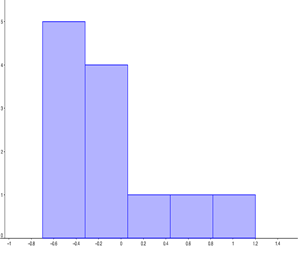
\includegraphics[width=0.3\textwidth]{./appendages/HP.png}
        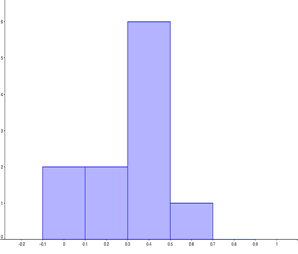
\includegraphics[width=0.3\textwidth]{./appendages/HC.png}
        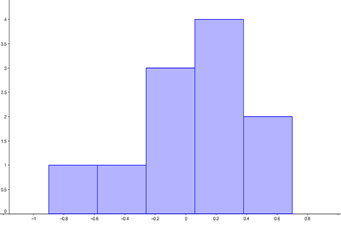
\includegraphics[width=0.3\textwidth]{./appendages/HF.png}
        \caption{Histogramas de piano, cello y flauta respectivamente. *Realizado en Geogebra.}
    \end{figure}
\end{center}
Los histogramas nos demuestran de forma gráfica que todas las muestras tienen distribuciones de frecuencias distintas.

%----------------------------------------------------------------------------------------
\subsection{Diagrama de caja y bigotes}
\begin{center}
    \begin{figure}[H]
        \centering
        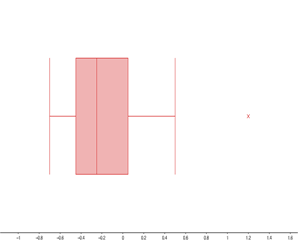
\includegraphics[width=0.3\textwidth]{./appendages/DBP.png}
        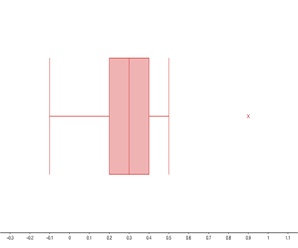
\includegraphics[width=0.3\textwidth]{./appendages/DBC.png}
        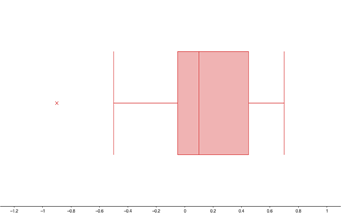
\includegraphics[width=0.3\textwidth]{./appendages/DBF.png}
        \caption{Diagrama de Caja y Bigotes de piano, cello y flauta respectivamente. *Realizado en Geogebra.}
    \end{figure}
\end{center}
El diagrama de caja es un método estandarizado para representar gráficamente una serie de datos numéricos a través de sus cuartiles. El diagrama es diferente para las tres muestras, con distinta variabilidad fuera de los cuartiles superior e inferior.

%----------------------------------------------------------------------------------------
\subsection{Normalidad}
\begin{center}
    \begin{figure}[H]
        \centering
        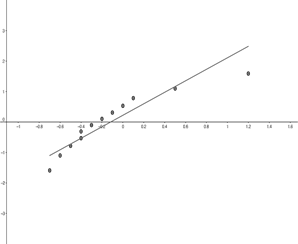
\includegraphics[width=0.3\textwidth]{./appendages/NP.png}
        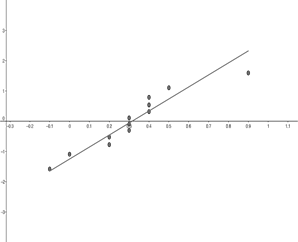
\includegraphics[width=0.3\textwidth]{./appendages/NC.png}
        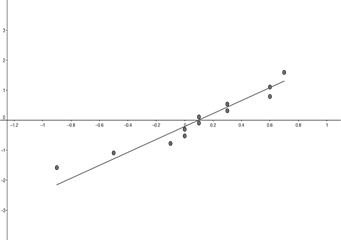
\includegraphics[width=0.3\textwidth]{./appendages/NF.png}
        \caption{Gráfica QQ de piano, cello y flauta respectivamente. *Realizado en Geogebra.}
    \end{figure}
\end{center}

Las muestras de las tres poblaciones no tienen normalidad. De esta forma, todas las pruebas que se podían realizar tenían que aceptar el supuesto de no normalidad. Por lo tanto, este proyecto de investigación utilizó únicamente pruebas de hipótesis no paramétricas.


\section{Discusión de resultados}
Tomando en cuenta el análisis de la base de datos y muestras de las poblaciones, se pudo realizar la prueba Kruskal-Wallis. Después de plantear las hipótesis, logramos rechazar la hipótesis nula y afirmar que las poblaciones son diferentes. A parte, pudimos determinar que las poblaciones de piano y cello son diferentes, así como pudimos observar que no tuvimos suficiente evidencia para decir que la población de cello y flauta son diferentes. Esto último tal vez podría tener un resultado distinto si se obtiene una muestra de mayor tamaño para estas dos poblaciones en específico.


Intuimos que estas diferencias entre las poblaciones se deben a las diferentes complejidades asociadas con tocar cada instrumento, considerando que los propios músicos están de acuerdo que hay instrumentos más difíciles que otros. Por lo que estas diferencias en dificultad pudieron haber causado las diferencias en los aumentos de dopamina. 



Puesto a estos resultados podría abrirse una nueva interrogante que plantee resolver qué instrumentos son los que estadísticamente tienden a segregar la mayor cantidad de dopamina posterior al ser tocados y cuales tienen la desventaja estadística de no segregar tanto, esta interrogante va más allá del enfoque de esta investigación por lo que podría tratarse en futuras investigaciones.


\section{Conclusiones}
\begin{enumerate}
    \item El tocar instrumentos en realidad si causa un cambio positivo en el nivel de dopamina, simplemente la magnitud del cambio no es la misma para el piano, cello y flauta.
    \item Hay evidencia suficiente para decir que la diferencia en niveles de dopamina para las  poblaciones de piano y cello no son iguales.
    \item No hay evidencia suficiente para decir que las poblaciones de cello y flauta son diferentes en términos de segregación de dopamina. 
    \item Aún sin que los datos tengan normalidad, o similar distribución de frecuencias, se pueden obtener hallazgos estadísticos fiables, gracias a las pruebas no paramétricas. 
\end{enumerate}


\section{Recomendaciones}
Tomando en consideración los resultados del proyecto de investigación y las conclusiones, se recomienda investigar otros aspectos relacionados con este tema:  

\begin{itemize}
    \item Cambios en los niveles de dopamina después de escuchar distintos géneros de música.
    \item Diferencia estadística de otros factores fisiológicos después de tocar los instrumentos más utilizados en el mundo de la música.
    \item Cual es el instrumento que estadísticamente causa una segregación más grande de dopamina.
    \item Cambios en niveles de otros neurotrasmisores después de tocar un instrumento.
\end{itemize}

A la hora de realizar el experimento y el trabajo de investigación, se recomienda fijar un rango de edades para los sujetos y realizar las pruebas alrededor de la misma hora del día, de forma de evitar sesgos externos en los resultados. Aunque no es necesaria la normalidad para la mayoría de pruebas, se recomienda que las muestras de todas las poblaciones sean $n\geq 7$ ($n_i\geq 5$ para Kruskal-Wallis \& $n\geq 7$ para Mann-Whitney-Wilcoxon y que las muestras sean independientes) de forma que se pueda usar mayor variedad de pruebas no paramétricas. 


Por último se recomienda realizar el procedimiento estadístico apoyándose de las herramientas de Excel y sus fórmulas, así como de Geogebra. Especialmente utilizar esta última para la generación rápida y fácil de distintas gráficas de los datos, como gráficas q-q, diagramas de caja e histogramas.


\section*{Herramientas utilizadas}
Se utilizaron las herramientas: 
\begin{itemize}
    \item Fórmulas de Excel.
    \item Calculadora de probabilidad de Geogebra.
    \item Hoja de Cálculos de Geogebra para realizar los cálculos.
    \item Lenguaje de programación Python con las librerias: \verb|random, requests| y el sitio web de random.org.
\end{itemize}



\section*{Bibliografía}

\begin{enumerate}[label={[\arabic*]}]
    \item \url{https://www.ncbi.nlm.nih.gov/pmc/articles/PMC4354683/pdf/nihms-667134.pdf }
    \item \url{https://www.eldiario.es/consumoclaro/cuidarse/principales-beneficios-tocar-instrumento-musical_1_1138883.html  }
    \item \url{https://www.mascaraquemarketing.com/el-cerebro-de-los-musicos/ }
    \item \url{https://www.muyinteresante.es/salud/articulo/ipor-que-es-la-musica-nos-provoca-placer }
    \item \url{https://psicologiaymente.com/neurociencias/hipocampo }
    \item \url{https://www.formulamedica.com.co/no-dejes-de-leer/tocar-un-instrumento-estimula-la-creatividad-mejora-la-habilidad-del-lenguaje-la-memoria-y-la-capacidad-de-atencion/ }
  \end{enumerate}


\end{document}

